\chapter{Cơ sở lý thuyết}
\label{chapter2}
Chương này em sẽ trình bày những kiến thức và các công cụ cần có để xây dựng một website
\section{Ngôn ngữ lập trình C\# } \label{ngonngu} 
C\# là một ngôn ngữ lập trình hướng đối tượng được phát triển bởi Microsoft, là phần khởi đầu cho kế hoạch .NET của Microsoft. Tên của ngôn ngữ bao gồm ký tự thăng theo Microsoft nhưng theo ECMA là C\#, chỉ bao gồm dấu số thường. Microsoft phát triển C\# dựa trên C++ và Java. C\# được miêu tả là ngôn ngữ có được sự cân bằng giữa C++, Visual Basic, Delphi và Java.

C\# được thiết kế chủ yếu bởi Anders Hejlsberg kiến trúc sư phần mềm nổi tiếng với các sản phẩm Turbo Pascal, Delphi, J++, WFC.
Tiêu chuẩn ECMA liệt kê các mục tiêu của việc thiết kế ngôn ngữ C\#:
\begin{itemize}
\item Ngôn ngữ được dự định là một ngôn ngữ lập trình đơn giản, hiện đại, hướng đến nhiều mục đích sử dụng, và là một ngôn ngữ lập trình hướng đối tượng.
\item Ngôn ngữ và việc triển khai đáp ứng các nguyên tắc của ngành kỹ thuật phần mềm như kiểm tra chặt chẽ kiểu dữ liệu, kiểm tra giới hạn mảng, phát hiện các trường hợp sử dụng các biến chưa có dữ liệu, và tự động thu gom rác. Tính mạnh mẽ, sự bền bỉ, và năng suất của việc lập trình là rất quan trọng đối với ngôn ngữ này.
\item Ngôn ngữ sẽ được sử dụng để phát triển các thành phần của phần mềm theo hướng thích hợp cho việc triển khai trong các môi trường phân tán.
\item Khả năng di chuyển (portability) là rất quan trọng, đặc biệt là đối với những lập trình viên đã quen với C và C++.
\item Hỗ trợ quốc tế hóa.
\item Ngôn ngữ sẽ được thiết kế để phù hợp với việc viết các ứng dụng cho cả hai hệ thống: hosted và nhúng, từ các phần mềm quy mô lớn, đến các phần mềm chỉ có các chức năng đơn giản.
\item Mặc dù các ứng dụng C\# có tính kinh tế đối với các yêu cầu về bộ nhớ và chế độ xử lý, ngôn ngữ này không cạnh tranh trực tiếp về hiệu năng và kích thước đối với ngôn ngữ C hoặc assembly
\item C\# được biên dịch ra mã trung gian MSIL sau đó thực thi bởi Common Language Runtime (CLR) \cite{2}.
\end{itemize}
\par
Em chọn ngôn ngữ C\# bởi vì:
\begin{itemize}
\item Rất phổ biến và được sử dụng bởi hàng triệu lập trình viên trên toàn thế giới.
\item Dễ học và sử dụng.
\item So với Java thì nó là đối thủ lớn nhất. Chúng ta không so sánh 2 ngôn ngữ nhưng em thích C\# vì nó luôn cải tiến.
\item Nền tảng .NET cũng luôn phát triển ngày càng hiện đại trong khi Java phát triển chậm.
\end{itemize}

\section{.NET}
.NET bao gồm 3 thành phần:
\begin{itemize}
\item Runtime
\item Libraries
\item Toolings
\end{itemize}
\par
Quy trình biên dịch và chạy chương trình của .NET. Hình \ref{refhinh2_2} ta thấy từ source code qua trình biên dịch tương ứng của ngôn ngữ đấy trong hệ sinh thái .NET ví dụ như C\# compiler hay VB.NET compiler để sinh ra MSIL code. Trong .Net ngôn ngữ trung gian trong .NET nó khá gần với mã máy những không chứa thông tin cụ thể về CPU, nên ngôn ngữ MSIL giúp cho đoạn code trung gian của chúng ta có thể hoạt động trên nhiều loại CPU (64bit, 32bit), cũng như nhiều loại kiến trúc khác nhau (ARM, Intel…). Trên thực tế một vài ngôn ngữ (Javascript, Python…) không sử dụng đến ngôn ngữ trung gian: Source sẽ được dịch thẳng ra mã máy tại tại ‘Runtime’. Điểm lợi của việc này là quá trình build được đơn giản hóa, tuy nhiên hiệu năng sẽ bị hạn chế.
Ngoài việc biên dịch, môi trường hoạt động (Runtime) còn có những công dụng như:
\begin{itemize}
\item Tự động quản lý bộ nhớ. Khi làm việc với những ngôn ngữ bậc cao như C\# hay Java, chúng ta không cần  giải phóng bộ nhớ bằng cách gọi free() như khi làm việc với C/C++. CLR bao gồm một công cụ dọn rác (Garbage collector -GC) sẽ tự động giải phóng những phần bộ nhớ không được sử dụng
\item Strong typings: CLR quản lý thông tin về các kiểu dữ liệu đã sử dụng. Điều này giúp cho lập trình viên có thể phân biệt được các định dạng thông tin của từng biến khác nhau (class, structure…)
\end{itemize}
Khi làm việc với .NET, code của chúng ta sẽ tương tác với rất nhiều các class khác nhau. Tất cả những class này được định nghĩa trong hệ thống thư viện cơ bản của .NET được gọi tắt là BCL (Base class libraries). Mã nguồn của BCL, trái với mọi người hay nghĩ, là mã nguồn mở. Chúng ta có thể truy cập mã nguồn này tại sourceof.net. Các công cụ (toolings) của .NET bao gồm compiler và Visual Studio .NET sử dụng hệ thống build của Microsoft gọi là MSBuild. Đối với nền tảng .NET core mới thì chúng ta còn có thêm công cụ dòng lệnh (dotnet cli).
\begin{center}
    \begin{figure}[h]
    \begin{center}
     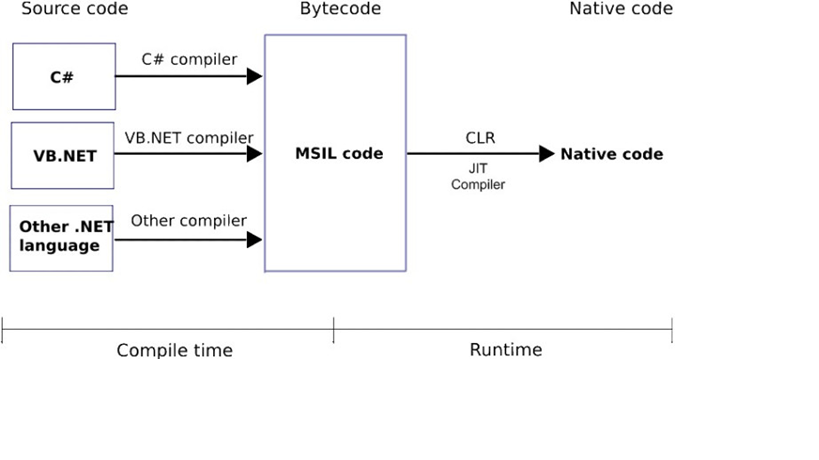
\includegraphics[scale=0.6]{image/chayDotNet.png}
    \end{center}
    \caption{Quy trình biên dịch và chạy chương trình}
    \label{refhinh2_2}
    \end{figure}
\end{center}
Hình \ref{refhinh2_3} chúng ta có thể thấy về cơ bản, .NET Framework, .NET core và Mono là ba phiên bản .NET khác nhau (có nghĩa là mỗi phiên bản có Runtime, Libraries và Toolings riêng).
\begin{center}
    \begin{figure}[h]
    \begin{center}
     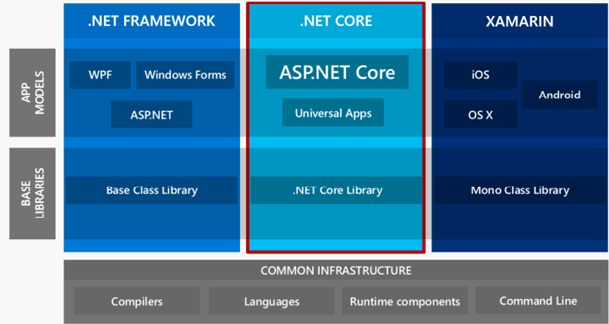
\includegraphics[scale=0.9]{image/kienTrucDotNetCore.png}
    \end{center}
    \caption{Kiến trúc của .NET }
    \label{refhinh2_3}
    \end{figure}
\end{center}
\begin{itemize}
\item .NET Framework được Microsoft đưa ra chính thức từ năm 2002. .NET Framework chỉ hoạt động trên Windows. Những nền tảng ứng dụng như WPF, Winforms, ASP.NET(1-4) hoạt động dựa trên .NET Framework.
\item Mono là phiên bản cộng đồng nhằm mang .NET đến những nền tảng ngoài Windows. Mono được phát triển chủ yếu nhằm xây dựng những ứng dụng với giao diện người dùng và được sử dụng rất rộng rãi: Unity Game, Xamarin…
\item Cho đến năm 2013, Microsoft định hướng đi đa nền tảng và phát triển .NET core. .NET core hiện được sử dụng trong các ứng dụng Universal Windows platform và ASP.NET Core.
\item Tuyệt đối không nên dùng Mono để vận hành web server. Bộ máy dọn rác của Mono không được thiết kế để hoạt động với webserver và sẽ gây ra quá tải nhanh chóng
\item Nên lựa chọn .NET Framework hay .NET Core cho các web server .NET Core chạy được đa nền tảng và có hiệu năng cao hơn. Nhược điểm duy nhất của nó là số lượng thư viện hỗ trợ vẫn còn hạn chế. .NET Framework có hệ sinh thái lớn hơn với nhiều các thư viện hỗ trợ hơn.
\end{itemize}

\subsection{.NET Framework}
Như đã nêu ở phần \ref{ngonngu} ngôn ngữ C\# ra đời để phục vụ Microsoft phát triển nền tảng .NET Framework phục vụ phát triền cho nhiều ứng dụng cho nên C\# không đứng riêng lẻ mà nó là 1 phần của nền tảng .NET, .NET Framework bao gồm môi trường phát triển, hỗ trợ đa ngôn ngữ mà C\# là một trong số đó (ngoài ra có F\#, VB.NET, Managed C++, J\#).
Những thành phần của .NET Framework (Hình \ref{refhinh2_1}) bao gồm:
\begin{itemize}
\item Các ngôn ngữ lập trình .NET (C\#, VB.NET…).
\item Môi trường thực thi code (CLR) sẽ thực thi chương trình được viết từ ngôn ngữ lập trình.
\item Các công cụ phát triển như trình biên dịch csc dung để biên dịch ngôn ngữ C\# sang mã trung gian (MSIL) mà CLR có thể hiểu.
\item Tập các thư viện chuẩn (Class Library) như ADO.NET cho phép truy cập database (ví dụ SQL Server hoặc MySQL) và WCF cho phép tạo ra các ứng dụng API theo chuẩn HTTP và trả về JSON, SOAP…
\end{itemize}
\begin{center}
    \begin{figure}[h]
    \begin{center}
     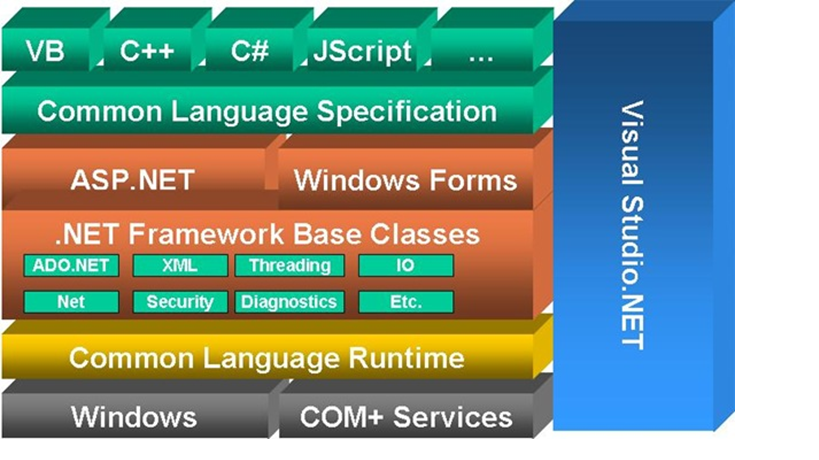
\includegraphics[scale=0.6]{image/kienTrucDotNet.png}
    \end{center}
    \caption{Kiến trúc .Net Framework}
    \label{refhinh2_1}
    \end{figure}
\end{center}
\subsection{Mono}
Mono là một nền tảng open-source với mục đích chính là tạo những ứng dụng cross-platform trên nền .Net. Bạn có thể sử dụng Mono trên các hệ điều hành như Unix, Linux, Mac OS X, Solaris và tất nhiên là Windows. Bất kì ngôn ngữ nào được biên dịch thành mã IL thuần túy đều có thể tương thích với Mono. Ngoài ra, Mono còn cung cấp thư viện hỗ trợ rất nhiều loại ngôn ngữ lập trình khác như Java, PHP, Python, Object Pascal, Cobra… Mono framework được sử dụng để lập trình ứng dụng mobile và game 2D, 3D. Các thành phần chính của Mono Framework:
\begin{itemize}
\item Mono runtime: cung cấp trình biên dịch Just-in-Time (JIT), Ahead-of-Time (AOT), thực thi, quản lý các tiến trình và giao tiếp với hệ thống.
\item C\# Compiler: bao gồm các công cụ
\begin{itemize}
\item mcs: (phiên bản 1.1) hỗ trợ C\# 1.0 và C\# 3.0 ngoại trừ các tính năng về generic.
\item gmcs: (phiên bản 2.0) hỗ trợ đầy đủ C\# 3.0.
\item smcs: (phiên bản 2.1) hỗ trợ thêm Silverlight/Moonlight.
\item dmcs: (phiên bản 4.0) hỗ trợ C\# 4.0.
\end{itemize}
\item Base Class Library: thư viện nền tảng để phát triển ứng dụng, tương thích với .Net framework.
\item Mono Class Library: Cung cấp các thư viện lập trình như Gtk+, Zip files, LDAP, OpenGL, Cairo, POSIX,… \cite{4}
\end{itemize}
\subsection{.NET Core}
.NET Core là một framework mã nguồn mở mới và framework đa nền tảng (cross-platform) cho việc xây dựng những ứng dụng hiện tại dựa trên kết nối đám mây, giống như web apps, IoT và backend cho mobile. Ứng dụng ASP.NET Core có thể chạy trên .NET Core hoặc trên phiên bản đầy đủ của .NET Framework. Nó được thiết kế để cung cấp và tối ưu hệ thống đang và đã phát triển cho những ứng dụng được triển khai trên đám mây (cloud) hoặc chạy on-promise. Nó bao gồm các thành phần theo hướng module nhằm tối thiểu tài nguyên và chi phí phát triển. Chúng ta có thể phát triển và chạy những ứng dụng ASP.NET Core đa nền tảng trên Windows, Mac và Linux. Đồng thời nó đã trở thành một mã nguồn mở. Đây là một thay đổi rất lớn và theo em là quan trọng nhất của ASP.NET Core. Điều mà trước đây khó có một lập trình viên nào có thể nghĩ đến. Có lẽ đó cũng là một xu thế mà các ngôn ngữ lập trình hiện nay đang hướng tới.
\par
Bản phát hành đầu tiên của ASP.NET đã xuất hiện cách đây 15 năm trước, nó là một phần của .NET Framework. Từ đó, hàng triệu lập trình viên đã sử dụng nó để xây dựng những ứng dụng web tuyệt vời, và trên những năm đó Microsoft đã phát triển thêm nhiều tính năng mới.ASP.NET Core có một số thay đổi kiến trúc lớn, đó là kết quả của việc học hỏi rất nhiều từ các framework module hóa khác. ASP.NET Core không còn dựa trên System.Web.dll nữa. Nó được dựa trên một tập hợp các gói, các module hay cũng được gọi là các Nuget packages. Điều này cho phép bạn tối ưu ứng dụng của bạn để chỉ bao gồm những packages nào cần thiết. Lợi ích của nó là giúp cho ứng dụng nhỏ hơn, bảo mật chặt chẽ hơn, giảm sự phức tạp, tối ưu hiệu suất hoạt động và giảm chi phí, thời gian cho việc phát triển.
Với ASP.NET Core bạn đạt được những nền tảng cải tiến dưới đây:
\begin{itemize}
\item Hợp nhất việc xây dựng web UI và web APIs.
\item Tích hợp những client-side frameworks hiện đại và những luồng phát triển.
\item Hệ thống cấu hình dựa trên môi trường đám mây thật sự.
\item Dependency injection được xây dựng sẵn.
\item HTTP request được tối ưu nhẹ hơn.
\item Có thể host trên IIS hoặc self-host trong process của riêng project hiện tại.
\item Được xây dựng trên .NET Core, hỗ trợ thực sự app versioning.
\item Chuyển các thực thể, thành phần, module như những NuGet packages
\item Những công cụ mới để đơn giản hóa quá trình phát triển web hiện đại
\item Xây dựng và chạy đa nền tảng(Windows, Mac và Linux)
\item Mã nguồn mở và tập trung vào cộng đồng
\end{itemize}

\subsection{Entity Framework Core}
\subsection{ASP.NET Identity}
\section{CSHTML}
CSHTML là 1 view engine dùng để xử lý và tạo HTML, nó là 1 view để nhận các dữ liệu mà controller gửi đến, CSHTML cho phép viết mã nguồn C\# để xử lý dữ liệu trên view dễ dàng hơn. CSHTML sử dụng Raroz để viết mã. Cơ chế Razor giảm thiểu số lượng ký tự và phím nhấn cần để tạo một tập tin View, do đó lập trình viên có thể làm việc nhanh và trôi chảy hơn. Khi chạy trên môi trường web thì file CSHTML sẽ tự động trở thành mã HTML để hiển thị lên các trình duyệt website
\section{Bootstrap}
Bootstrap là 1 framework HTML, CSS, và JavaScript cho phép người dùng dễ dàng thiết kế website theo 1 chuẩn nhất định, tạo các website thân thiện với các thiết bị cầm tay như mobile, ipad, tablet,...
\par
Bootstrap bao gồm những cái cơ bản có sẵn như: typography, forms, buttons, tables, navigation, modals, image carousels và nhiều thứ khác. Trong bootstrap có thêm nhiều Component, Javascript hỗ trợ cho việc thiết kế reponsive của bạn dễ dàng, thuận tiện và nhanh chóng hơn. Nên dùng bootstrap để viết giao diện front-end vì:
\begin{itemize}
\item Bootstrap là một trong những framework được sử dụng nhiều nhất trên thế giới để xây dựng nên một website. Bootstrap đã xây dựng nên 1 chuẩn riêng và rất được người dùng ưa chuộng. Chính vì thế, chúng ta hay nghe tới một cụm từ rất thông dụng "Thiết kế theo chuẩn Bootstrap".
\item Rất dễ để sử dụng: Nó đơn giản vì nó được base trên HTML, CSS và Javascript chỉ cẩn có kiến thức cơ bản về 3 cái đó là có thể sử dụng bootstrap tốt.
\item Responsive: Bootstrap xây dựng sẵn reponsive css trên các thiết bị Iphones, tablets, và desktops. Tính năng này khiến cho người dùng tiết kiệm được rất nhiều thời gian trong việc tạo ra một website thân thiện với các thiết bị điện tử, thiết bị cầm tay.
\item Tương thích với trình duyệt: Nó tương thích với tất cả các trình duyệt (Chrome, Firefox, Internet Explorer, Safari, and Opera). Tuy nhiên, với IE browser, Bootstrap chỉ hỗ trợ từ IE9 trở lên. Điều này vô cùng dễ hiểu vì IE8 không support HTML5 và CSS3.
\end{itemize}

\section{Jquery Ajax}
\subsection{Jquery}
jQuery là một Framework được xây dựng dựa trên các tính năng của JavaScript. Vì thế trong khi phát triển các ứng dụng sử dụng jQuery, bạn có thể sử dụng tất cả các hàm và các tính năng khác được bổ trợ trong JavaScript. jQuery làm đơn giản hóa việc truyền tải HTML, xử lý sự kiện, tạo hiệu ứng động và tương tác Ajax. Với jQuery, khái niệm Rapid Web Development đã không còn quá xa lạ. jQuery là một bộ công cụ tiện ích JavaScript làm đơn giản hóa các tác vụ đa dạng với việc viết ít code hơn. Dưới đây liệt kê một số tính năng tối quan trọng được hỗ trợ bởi jQuery:
\begin{itemize}
\item Thao tác DOM: jQuery giúp dễ dàng lựa chọn các phần tử DOM để traverse (duyệt) một cách dễ dàng như sử dụng CSS, và chỉnh sửa nội dung của chúng bởi sử dụng phương tiện Selector mã nguồn mở, mà được gọi là Sizzle.
\item Xử lý sự kiện: jQuery giúp tương tác với người dùng tốt hơn bằng việc xử lý các sự kiện đa dạng mà không làm cho HTML code rối tung lên với các Event Handler.
\item Hỗ trợ AJAX: jQuery giúp bạn rất nhiều để phát triển một site giàu tính năng và phản hồi tốt bởi sử dụng công nghệ AJAX.
\item Hiệu ứng: jQuery đi kèm với rất nhiều các hiệu ứng đa dạng và đẹp mắt mà bạn có thể sử dụng trong các Website của mình.
\item Gọn nhẹ: jQuery là thư viện gọn nhẹ - nó chỉ có kích cỡ khoảng 19KB (gzipped).
\item Được hỗ trợ hầu hết bởi các trình duyệt hiện đại: jQuery được hỗ trợ hầu hết bởi các trình duyệt hiện đại, và làm việc tốt trên IE 6.0+, FF 2.0+, Safari 3.0+, Chrome và Opera 9.0+
\end{itemize}


    \begin{longtable}{m{0.1\linewidth}  m{0.3\linewidth}  m{0.5\linewidth}}
    \caption{Các hàm có sẵn trong Jquery \cite{3}} \\ \hline
     	\textbf{STT} & \textbf{Tên hàm} & \textbf{Mô tả hàm} \\ \hline
     	1&charAt()&Trả về ký tự tại chỉ mục (index) đã cho. \\
		\hline
     	2&concat()&Kết nối hai chuỗi văn bản và trả về một chuỗi mới.\\
		\hline
     	3&forEach()&Gọi một hàm cho mỗi phần tử của một mảng.\\
     	\hline
     	4&indexOf()&Trả về chỉ mục về sự xuất hiện đầu tiên bên trong việc gọi đối tượng String với giá trị đã cho, hoặc -1 nếu không tìm thấy.\\
     	\hline
     	5&length()&Trả về độ dài của chuỗi.\\
     	\hline
     	6&pop()&Gỡ bỏ phần tử cuối của một mảng và trả về phần tử đó.\\
     	\hline
		7&push()&Thêm một hoặc nhiều phần tử tới phần cuối của một mảng và trả về độ dài mới của mảng đó.\\
		\hline
		8&reverse()&Đảo ngược thứ tự các phần tử trong một mảng – phần tử đầu tiên thành cuối cùng và cuối cùng thành đầu tiên.\\
		\hline
		9&sort()&Sắp xếp phân loại các phần tử của một mảng.\\
		\hline
		10&substr()&Trả về các ký tự trong một mảng bắt đầu từ vị trí đã cho từ số các ký tự đã xác định.\\
		\hline
		11&toLowerCase()&Trả về giá trị chuỗi đang gọi được biến đổi thành kiểu chữ thường.\\
		\hline
		12&toString()&Trả về sự biểu diễn chuỗi của giá trị số.\\
		\hline
		13&toUpperCase()&Trả về giá trị chuỗi đang gọi được biến đổi thành chữ hoa. \\ \hline
	\label{bang2_1}
    \end{longtable}
\subsection{Ajax}
Ajax là một bộ công cụ cho phép load dữ liệu từ server mà không yêu cầu tải lại trang.Nó sử dụng chức năng sẵn có XMLHttpRequest(XHR) của trình duyệt để thực hiện một yêu cầu đến server và xử lý dữ liệu server trả về.
\par
\textit{Ví dụ} : khi một người dùng viết một nhận xét trên bài viết đăng trên trang Facebook. Sau khi người dùng gửi nhận xét thành công trang Facebook mà người đó đang truy cập cần phải được cập nhật để hiển thị nhận xét vừa mới được tạo ra này. Nếu load lại toàn bộ trang mà người dùng đang truy cập thì sẽ không hiệu quả do tất cả những gì chúng ta muốn là hiển thị nhận xét mới được tạo ra, Ajax được tạo ra để giải quyết vấn đề này, thay vì tải lại toàn bộ trang trình duyệt sẽ chỉ l những phần được thay đổi để tiết kiệm thời gian chờ đợi một lượng thông tin lớn về từ server.\par
Một số ứng dụng sử dụng Ajax như : Gmail , Google Maps , Youtube , Facebook,...\par
Jquery cung cấp một số phương thức để thực hiện các chức năng ajax. Chúng ta có thể yêu cầu các text, HTML, XML và JSON từ server sử dụng cả giao thức HTTP GET và HTTP POST, chúng ta cũng có thể lấy dữ liệu từ bên ngoài trực tiếp vào trong phần tử được chọn.
\begin{itemize}
\item  Phương thức jquery load()
\begin{lstlisting}
$(selector).load(URL,data,callback);
\end{lstlisting}
\begin{itemize}
\item URL: mà bạn muốn lấy dữ liệu.
\item Data: cặp key/value gửi đi cùng với yêu cầu.
\item Callback: tên của hàm sẽ được thực thi sau khi phương thức load hoàn thành.
\end{itemize}
\end{itemize}

 




